\chapter{\label{appx:rusltc_err}\textit{RusLTC} error taxonomy}
%\addcontentsline{toc}{chapter}{Appendix C. Core MQM taxonomy}

\begin{multicols}{2}

\noindent Hierarchical tags with frequencies% in error-annotated subcorpus

\begin{table}[H]
	\centering
	\begin{tabular}{lr}
		\toprule
		tag & number \\
		\midrule
		Content               & 136   \\
		\hspace{1em}content\_reference    & 380   \\
		\hspace{3em}omission              & 59    \\
		\hspace{3em}distortion            & 785   \\
		\hspace{3em}nonsense              & 391   \\
		\hspace{3em}inexact               & 340   \\
		\hspace{3em}unclear               & 549   \\
		\hspace{1em}content\_cohesion     & 429   \\
		\hspace{3em}theme-rheme            & 225   \\
		\hspace{3em}logic                 & 493   \\
		\hspace{1em}content\_pragmatics   & 454   \\
		\hspace{3em}register              & 186   \\
		\hspace{3em}use                   & 230   \\
		SUBTOTAL						  & 4657  \\
		\midrule
		Language              & 12    \\
		\hspace{1em}language\_lexical     & 467   \\
		\hspace{3em}choice-of-word        & 1879  \\
		\hspace{3em}combinability         & 1144  \\
		\hspace{1em}language\_morphology  & 87    \\
		\hspace{3em}wordform       & 226   \\
		\hspace{1em}language\_syntax      & 591   \\
		\hspace{3em}incomplete & 88    \\
		\hspace{3em}ungrammatical         & 333   \\
		\hspace{3em}word\_order           & 174   \\
		\hspace{3em}preposition           & 88    \\
		\hspace{3em}delete                & 552   \\
		\hspace{1em}language\_spelling    & 245   \\
		\hspace{3em}capitals              & 137   \\
		\hspace{3em}typo                  & 122   \\
		\hspace{1em}language\_punctuation & 545   \\
		SUBTOTAL						  & 6690  \\
		\midrule
		TOTAL                 & 11347 \\
		\bottomrule
	\end{tabular}
\caption{\label{tab:errstats}Distribution of error across categories}
\end{table}

\columnbreak

\vspace*{10em}
\noindent Error attributes assigned to spans

\begin{table}[H]
	\centering
	\begin{tabular}{lr}
		\toprule
		attribute & number \\
		\midrule
		Severities      &    \\
		\hspace{1em}critical         & 1159 \\
		\hspace{1em}major            & 3034 \\
		\hspace{1em}minor            & 7154  \\
		\midrule
		Technology       &      \\
		\hspace{1em}background\_info & 67   \\
		\hspace{1em}SL               & 81   \\
		\hspace{1em}TL               & 144  \\
		\hspace{1em}too\_literal     & 686  \\
		\hspace{1em}too\_free        & 59   \\
		\hspace{1em}proper\_name     & 144  \\
		\hspace{1em}inconsistency    & 17   \\
		Good\_job        & 713  \\
		\midrule
		AnnotatorNotes   & 5548 \\
		\bottomrule
	\end{tabular}
\caption{\label{tab:attstats}Distribution of error attributes}
\end{table}

\end{multicols}

\begin{sidewaysfigure}
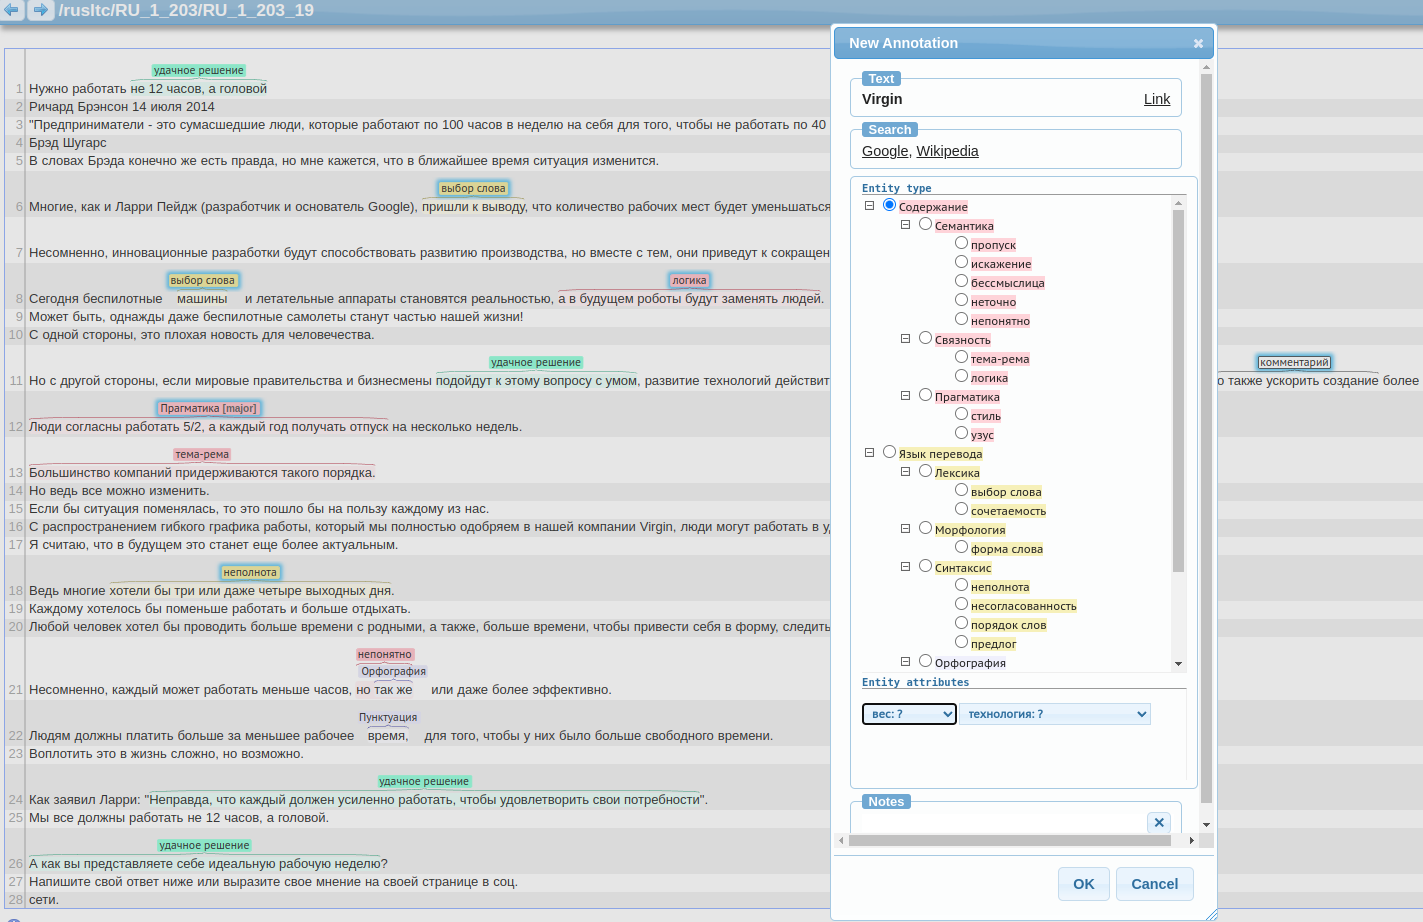
\includegraphics[width=\textwidth]{figures/brat}
\caption{\label{fig:brat}Screenshot of a \textit{brat}-based annotation environment}
\end{sidewaysfigure}

\begin{table}[H]
	\centering
	\begin{tabular}{lr}
		\toprule
		error type & weight \\
		\midrule
		Content               & 1   \\
		\hspace{1em}content\_reference    & 2   \\
		\hspace{3em}omission              & 2    \\
		\hspace{3em}distortion            & 3   \\
		\hspace{3em}nonsense              & 3   \\
		\hspace{3em}inexact               & 1   \\
		\hspace{3em}unclear               & 2   \\
		\hspace{1em}content\_cohesion     & 2   \\
		\hspace{3em}theme-rheme           & 1   \\
		\hspace{3em}logic                 & 3   \\
		\hspace{1em}content\_pragmatics   & 1   \\
		\hspace{3em}register              & 3   \\
		\hspace{3em}use                   & 2   \\
		\midrule
		Language              			  & 1    \\
		\hspace{1em}language\_lexical     & 1   \\
		\hspace{3em}choice-of-word        & 3  \\
		\hspace{3em}combinability         & 3  \\
		\hspace{1em}language\_morphology  & 1    \\
		\hspace{3em}wordform              & 1   \\
		\hspace{1em}language\_syntax      & 2   \\
		\hspace{3em}incomplete            & 3    \\
		\hspace{3em}ungrammatical         & 3   \\
		\hspace{3em}word\_order           & 2   \\
		\hspace{3em}preposition           & 3    \\
		\hspace{3em}delete                & 2   \\
		\hspace{1em}language\_spelling    & 1   \\
		\hspace{3em}capitals              & 1   \\
		\hspace{3em}typo                  & 1   \\
		\hspace{1em}language\_punctuation & 1   \\
		\bottomrule
	\end{tabular}
	\caption{\label{tab:errweights}Weights assigned to error categories for accuracy and fluency scores}
\end{table}
